%!TEX root = ../thesis.tex
\section{実験2:提案手法による人追従の実験}

  実験2では,提案手法による人追従の実験を行う.

\subsection{実験目的}

  提案手法により画像に基づいて人を追従する行動が生成されるかを,10回の実験により有効性を検証する.

\subsection{実験方法}

  実験では,学習フェーズの後に追従フェーズに移行する.以下にそれぞれの役割を示す.

  \subsubsection*{<学習フェーズ>}
  学習フェーズでは,追従対象者が再帰反射テープを装着し,\figref{Fig:RobotGuidance_course}における青色で示された場所(ホワイエ)を2DLiDARの最大検出範囲(120\, [deg])に注意しながら,10分間ランダムに歩き回る.

  \subsubsection*{<追従フェーズ>}
  追従フェーズでは,反射強度を利用していないことをわかりやすくするため,追従対象者は再帰反射テープを取り外す.また,学習フェーズとは異なり,\figref{Fig:RobotGuidance_course}における赤色で示されたコースを1周する.このコースは1周約90mであり,学習フェーズで学習したモデルを用いて,2DLiDARは使用せずに画像のみで人追従を行う.その時のロボットの挙動を確認する.

  \vspace{1cm}

  学習フェーズでの10分間の学習と追従フェーズでのテストコースを1周することを1セットとし,10セット実験を行った.

\newpage

  \begin{figure}[h]
    \centering
    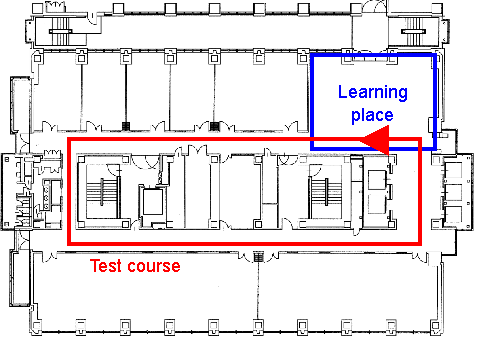
\includegraphics[keepaspectratio, scale=0.70] {images/pdf/RobotGuidance_course}
    \captionsetup{justification=raggedright} % キャプションを左寄せに
    \caption{Learning and following phase courses}
    \label{Fig:RobotGuidance_course}
  \end{figure}

\newpage

\subsection{結果と考察}

  すべての実験でロボットが人を追従する様子が確認できた.以下にそれぞれのフェーズの様子を記述する.

  \subsubsection*{<学習フェーズ>}
  
  学習フェーズにおける実験の様子を\figref{Fig:Learning phase in experiment}に示す.2DLiDARの反射強度を利用したルールベース制御器を使用することで学習フェーズにおいてロボットが人を追従する様子が確認できた.10セットの学習を行ったが,全てのセットにおいて人追従が途切れることはなかった.つまり,ルールベース制御器の有効性が確認できた.

  \begin{figure}[h]
    \centering
    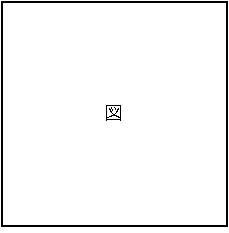
\includegraphics[keepaspectratio, scale=0.80] {images/pdf/figure}
    \captionsetup{justification=raggedright} % キャプションを左寄せに
    \caption{Learning phase in experiment}
    \label{Fig:Learning phase in experiment}
  \end{figure}

\newpage

  \subsubsection*{<追従フェーズ>}
  
  追従フェーズにおける実験の様子を\figref{Fig:Following phase in experiment}に示す.テストコースの道中で,追従対象者のビブスと同じ青色の壁紙が貼られていたが,そちらに釣られることなく人追従行動を継続する様子が確認できた.

  \begin{figure}[h]
    \centering
    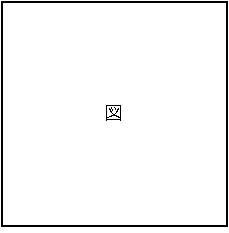
\includegraphics[keepaspectratio, scale=0.80] {images/pdf/figure}
    \captionsetup{justification=raggedright} % キャプションを左寄せに
    \caption{Following phase in experiment}
    \label{Fig:Following phase in experiment}
  \end{figure}

  実験結果を\tabref{tab:Experiment result}に示す.10回の試行中,9回は壁に衝突することなくコースを1周することができた.学習ステップ数は,0.2秒周期で学習して1stepとしているので,10分の学習で3000stepとなった.つまり,各学習モデルには3000個のデータが含まれ,人追従行動を明示的に学習せずに自動的に獲得している.一方で,10回の試行中,1回は\figref{Fig:RobotGuidance_failed_place}に示すように,テストコースの最初の曲がり角で壁に衝突した.失敗した場合の学習フェーズでの角速度のヒストグラムを\figref{Fig:Histogram of angular velocity}の(b)に示す.成功時の角速度のヒストグラムは(a)で,両者を比較すると,失敗時の左旋回の最大角速度が0.1\, [rad/s]小さいことがわかる.このことから,学習フェーズで0.3\, [rad/s]以上の角速度で左旋回する行動を学習していないのにもかかわらず,追従フェーズで0.3\, [rad/s]以上の角速度で左旋回しなければならない位置に追従対象者が立っていたことが原因で,曲がりきれずに壁に衝突してしまったと考えられる.ただし,これについてはさらなる調査が必要である.

  \begin{table}[h]
    \caption{Experiment result}
    \label{tab:Experiment result}
    \centering
    \begin{tabular}{|c|c|}
    \hline
    Step & Result      \\ \hline
    3000 & 9/10 (90\%) \\ \hline
    \end{tabular}
    \end{table}

\newpage

  \begin{figure}[h]
    \centering
    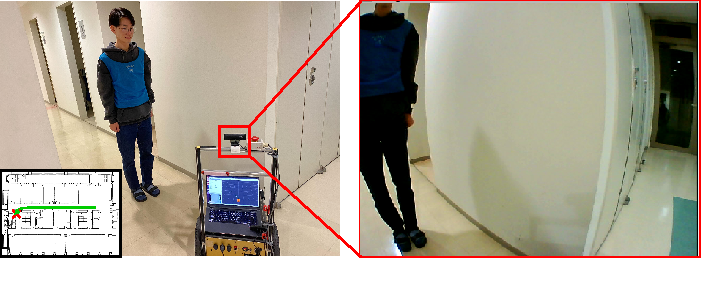
\includegraphics[keepaspectratio, scale=0.80] {images/pdf/RobotGuidance_failed_place}
    \captionsetup{justification=raggedright} % キャプションを左寄せに
    \caption{Failed at the first corner}
    \label{Fig:RobotGuidance_failed_place}
  \end{figure}

  \begin{figure}[h]
    \centering
    \begin{minipage}[c]{65mm} 
        \centering
        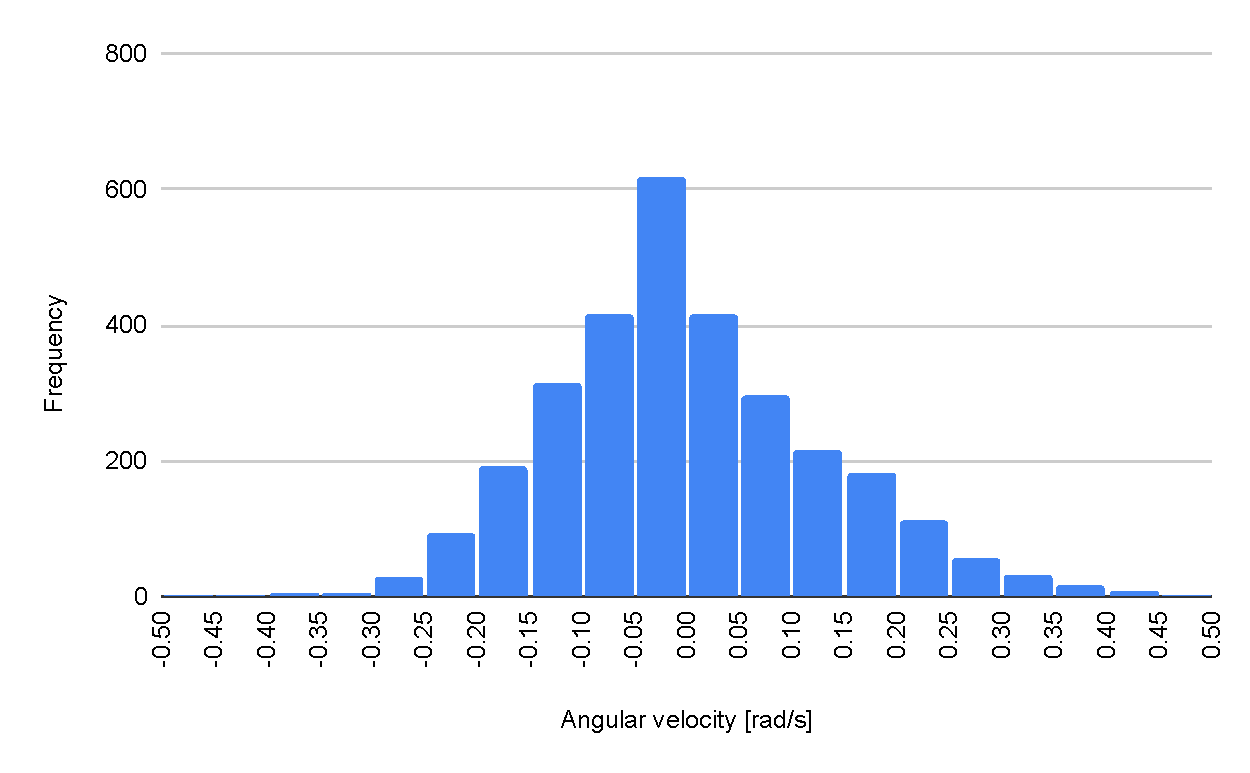
\includegraphics[height=45mm]{images/pdf/RobotGuidance_success_histogram}
        \subcaption{Success}
    \end{minipage}
    \begin{minipage}[c]{65mm} 
        \centering
        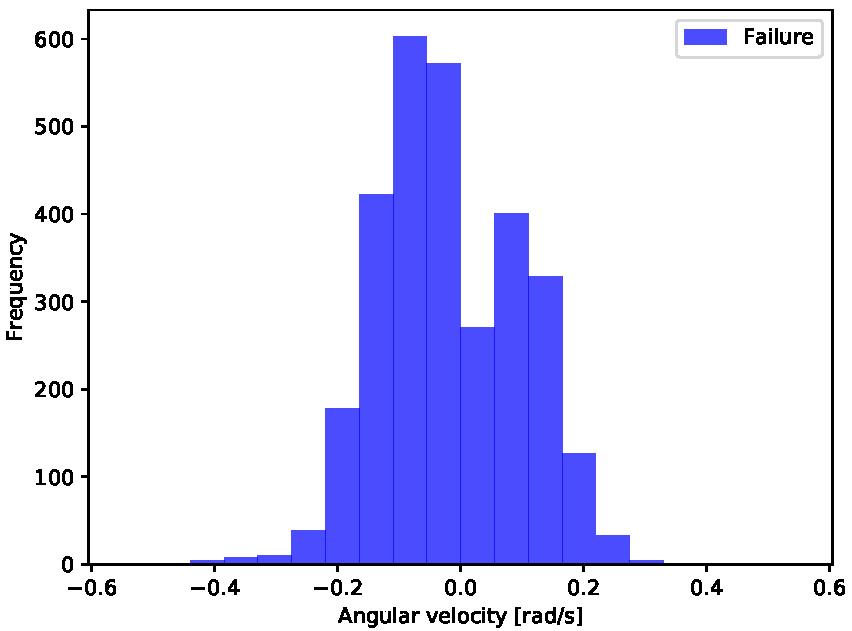
\includegraphics[height=45mm]{images/pdf/RobotGuidance_failed_histogram}
        \subcaption{Failure}
    \end{minipage}
    \caption{Histogram of angular velocity}
    \label{Fig:Histogram of angular velocity}
  \end{figure}

\newpage
